\section{Background}

\subsection{What is RCU?}

Read-copy update (RCU) is a synchronization mechanism
that is often used to replace reader-writer locking.
RCU readers run concurrently with updaters,
and so RCU avoids read-side contention by maintaining multiple versions of
objects and ensuring 
they are not freed until all pre-existing readers complete, that is,
until after a \emph{grace period} elapses.
The basic idea is to split updates into removal
and reclamation phases that are separated by a grace period~\cite{McKenneyRCU98}.
The removal phase removes reader-accessible references 
to objects, perhaps by replacing them with new versions.

Modern CPUs guarantee that writes to single aligned
pointers are atomic, so that readers
see either the old or new version of the data structure.
These atomic-write semantics enable atomic
insertions, deletions, and replacements in a linked structure.
This in turn enables readers to dispense with expensive
atomic operations, memory barriers, and cache misses.
In fact, in the most aggressive configurations of Linux-kernel RCU, readers
can use exactly the same sequence of instructions that would be used in
a single-threaded implementation, providing
RCU readers with excellent performance and scalability.

As illustrated in Figure~\ref{fig:rcu_concepts}, grace periods are only
needed for those readers whose runtime overlaps the removal phase.
Those that start after the removal 
phase cannot hold references to the removed objects and thus
cannot be disrupted by objects being freed during the reclamation phase.

\begin{figure}[tbp]
\centering
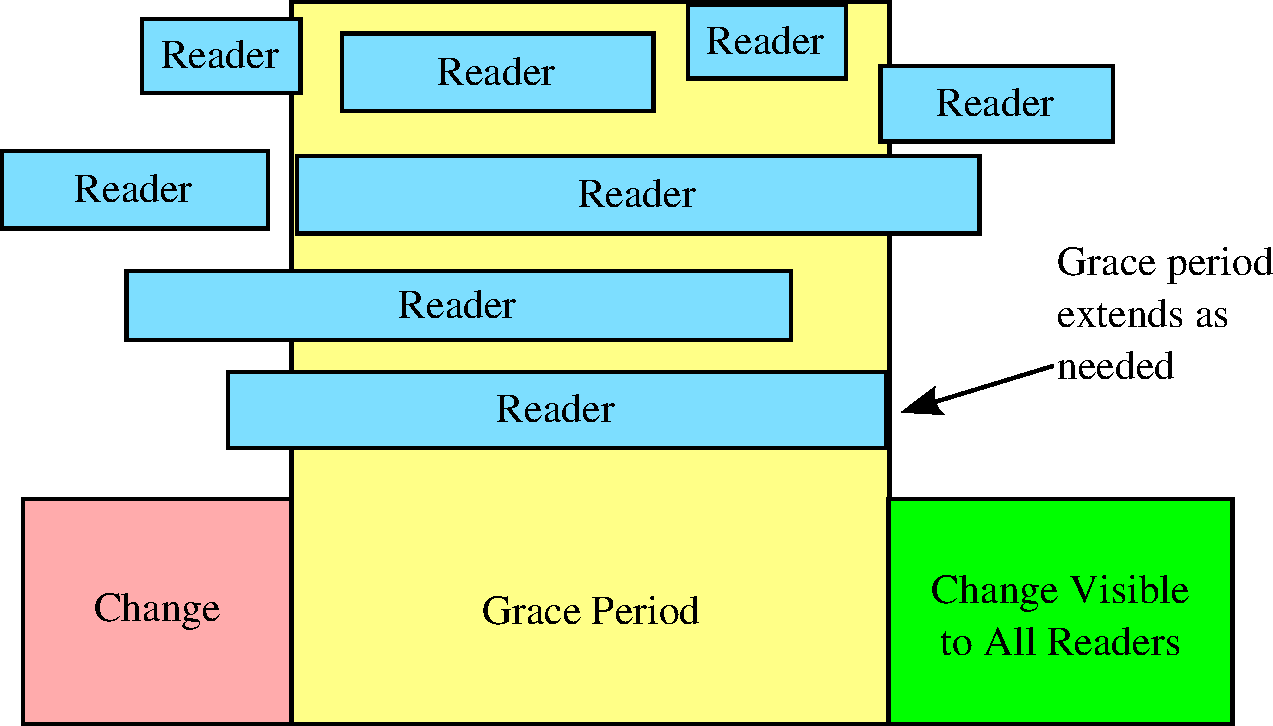
\includegraphics[scale=0.35]{rcu_concepts.pdf}
\caption{RCU Concepts}
\label{fig:rcu_concepts}
\end{figure}

\subsection{Программный интерфейс RCU} \label{sec:api_usage}
Программный интерфейс RCU достаточно невелик и состоит всего из пяти операций:
\co{rcu_read_lock()}, \co{rcu_read_unlock()}, \co{synchronize_rcu()},
\co{rcu_assign_pointer()}, and \co{rcu_dereference()}~\cite{McKenneyOSR08}.

Критическая секция RCU-читателя начинается с \co{rcu_read_lock()}
и заканчивается соответсвующим \co{rcu_read_unlock()}.
Вложенные критические секции чтения объединяются.
Внутри критической секции запрещается блокирование данного потока.
Данные, чтение которых осуществляется доступ внутри критической секции RCU,
будут доступны до её окончания.

Функция \co{synchronize_rcu()} соответсвует окончанию выполнения кода,
обновляющего значение объекта, тем самым сигнализируя о начале фазы освобождения.
Она блокирует поток-писатель до тех пор, пока все потоки-читатели
не выйдут из своих критических RCU-секций.
Отметим, что \co{synchronize_rcu()} не ожидает окончания
критических секций, вход в которые был осуществлен позже её вызова.

%\comment{Lihao: add example, e.g. http://paulmck.livejournal.com/39343.html}

\begin{figure}[tbp]
\centering
\footnotesize
\begin{verbatim}
               int x = 0;
               int y = 0;
               int r1, r2;

               void rcu_reader(void) {
                 rcu_read_lock();
                 r1 = x;
                 r2 = y;
                 rcu_read_unlock();
               }

               void rcu_updater(void) {
                 x = 1;
                 synchronize_rcu();
                 y = 1;
               }

               ...

               // after both rcu_reader()
               // and rcu_updater() return
               assert(r2 == 0 || r1 == 1);
\end{verbatim}
\caption{Verifying RCU Grace Periods}
\label{fig:verify_rcu_gp}
\end{figure}

Рассмотрим пример, приведенный на рисунке~\ref{fig:verify_rcu_gp}.
Если вход в критическую секцию чтения функции \co{rcu_reader()} выполнится до
вызова \co{synchronize_rcu()} в \co{rcu_updater()}, то выход из ней должен быть
совершен до возврата из \co{synchronize_rcu()}, чтобы значение переменной
\co{r2} было равно 0. Если же вход в неё произойдет после возврата из
\co{synchronize_rcu()}, то значение \co{r1} будет равным 1.

Наконец, для присвоения нового значения указателю, защищенному RCU,
потоки-писатели должны использовать \co{rcu_assign_pointer()},
которая возвращает новое значение.
RCU-читатели могут использовать \co{rcu_dereference()} для чтения
указателя, защищенного RCU, который впоследствии может быть безопасно разыменован.
%Note that this API does not actually dereference the pointer.
%Instead, it only fetches the pointer for later dereferencing.
Возвращаемое ею значение является корректным лишь внутри критической секции.
% Lihao: include this in PhD thesis and the technical report
Функции \co{rcu_assign_pointer()} и \co{rcu_dereference()} используются в паре
для того, чтобы убедиться, что если данный поток-читатель разыменовывает
защищенный указатель на только что вставленный объект, операция разыменования
вернет корректное значение, а не недоинициализированный мусор.

